\newpage
\section*{Anexo C: Resultados}
\addcontentsline{toc}{section}{Anexo C: Resultados} \label{AnexoC}

\subsection*{Resultados análisis de multifractalidad}
\addcontentsline{toc}{subsection}{Resultados análisis de multifractalidad}


\begin{figure}[!htb]
    \begin{minipage}{0.48\textwidth}
        \centering
        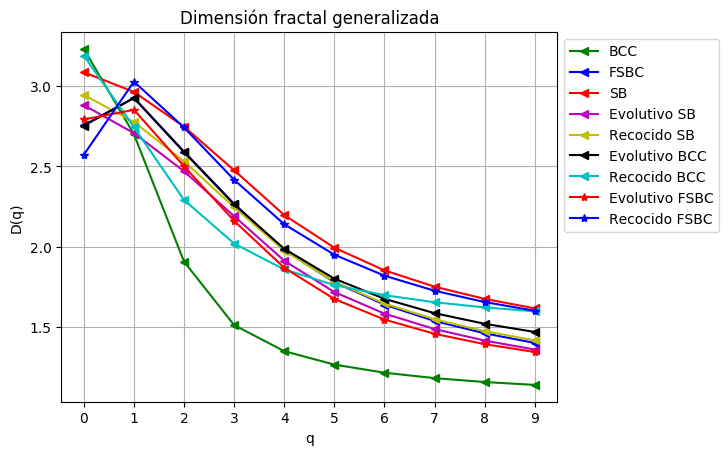
\includegraphics[scale=0.5]{CapituloAAnexos/imagenesAnexoC/Fractalidad/grafica_Dq20180502_203759ScaleFree2000Nodes.png}
        \caption{Análisis multifractal red libre de escala 2000 nodos}
    \end{minipage}\hfill
   \begin{minipage}{0.48\textwidth}
         \centering
        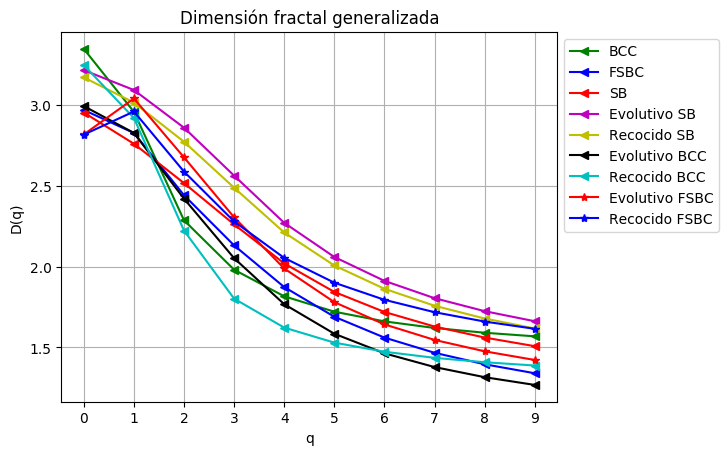
\includegraphics[scale=0.5]{CapituloAAnexos/imagenesAnexoC/Fractalidad/grafica_Dq20180506_035455ScaleFree4000Nodes.png}
    \caption{Análisis multifractal red libre de escala 4000 nodos}
    \end{minipage}
\end{figure}


\begin{figure}[!htb]
    \begin{minipage}{0.48\textwidth}
        \centering
        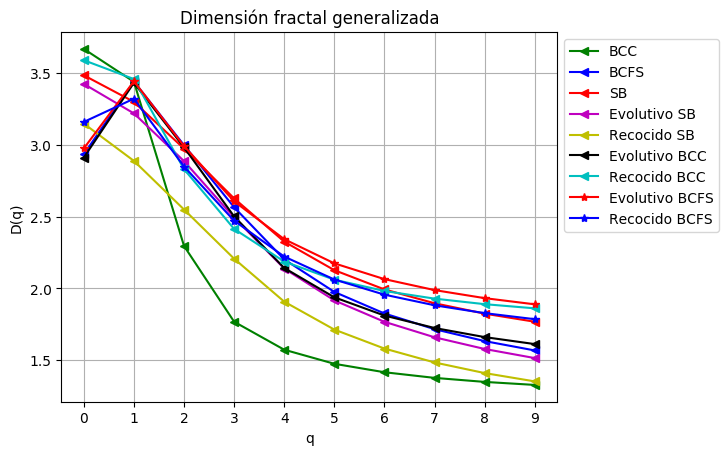
\includegraphics[scale=0.5]{CapituloAAnexos/imagenesAnexoC/Fractalidad/grafica_Dq20180525_061308ScaleFree8000Nodes.png}
    \caption{Análisis multifractal red libre de escala 8000 nodos}
    \end{minipage}\hfill
   \begin{minipage}{0.48\textwidth}
         \centering
        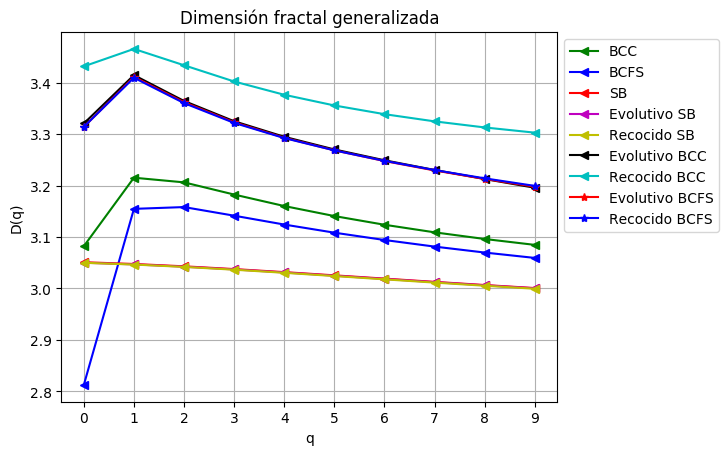
\includegraphics[scale=0.5]{CapituloAAnexos/imagenesAnexoC/Fractalidad/grafica_Dq20180509_024709SmallWorld5000NodesRewire005.png}
    \caption{Análisis multifractal Mundo pequeño p=5\%}
    \end{minipage}
\end{figure}

\begin{figure}[!htb]
    \begin{minipage}{0.48\textwidth}
        \centering
        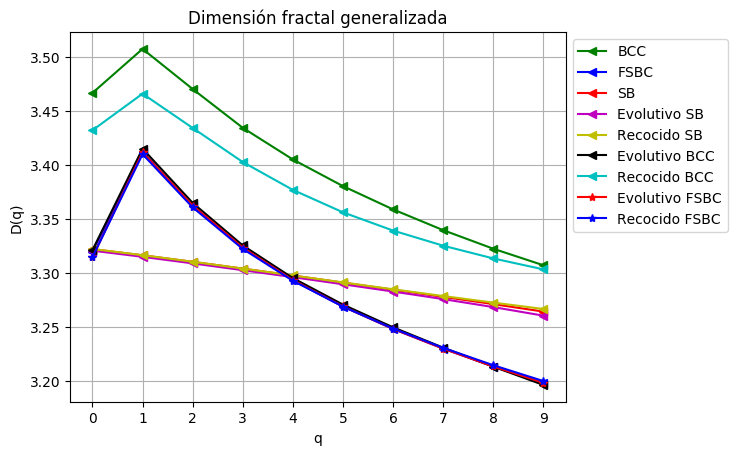
\includegraphics[scale=0.5]{CapituloAAnexos/imagenesAnexoC/Fractalidad/grafica_Dq20180506_141058SmallWorld5000NodesRewire01.png}
        \caption{Análisis multifractal Mundo pequeño p=10\%}
    \end{minipage}\hfill
   \begin{minipage}{0.48\textwidth}
         \centering
        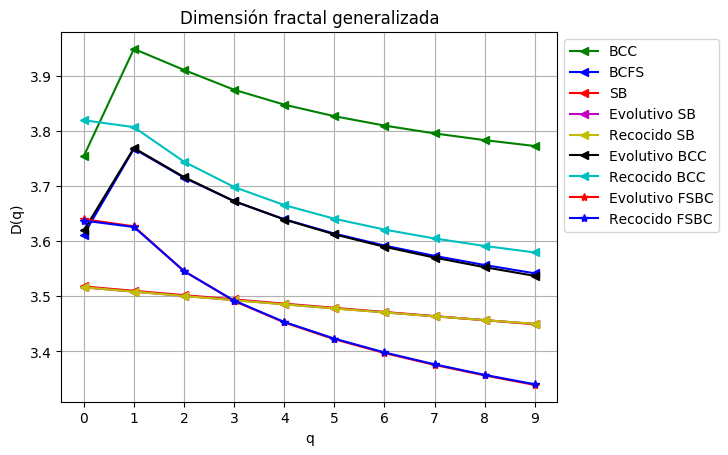
\includegraphics[scale=0.5]{CapituloAAnexos/imagenesAnexoC/Fractalidad/grafica_Dq20180505_223804SmallWorld5000NodesRewire02.png}
    \caption{Análisis multifractal Mundo pequeño p=20\%}
    \end{minipage}
\end{figure}


\begin{figure}[!htb]
    \begin{minipage}{0.48\textwidth}
        \centering
        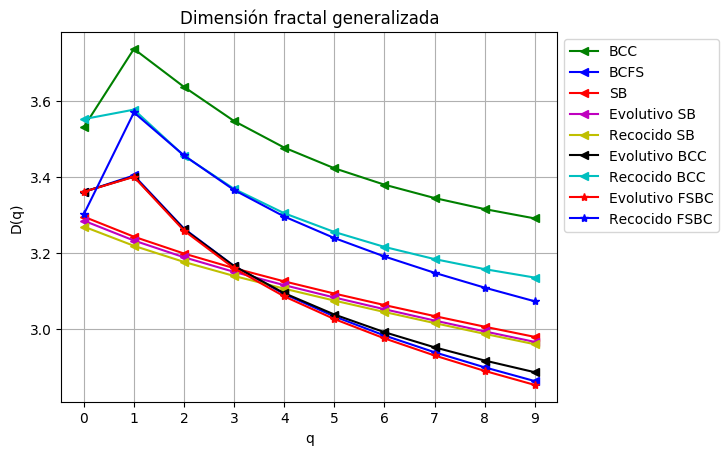
\includegraphics[scale=0.5]{CapituloAAnexos/imagenesAnexoC/Fractalidad/grafica_Dq20180502_133953Random1991Nodes5939.png}
        \caption{Análisis multifractal red aleatoria 1991 nodos}
    \end{minipage}\hfill
   \begin{minipage}{0.48\textwidth}
         \centering
        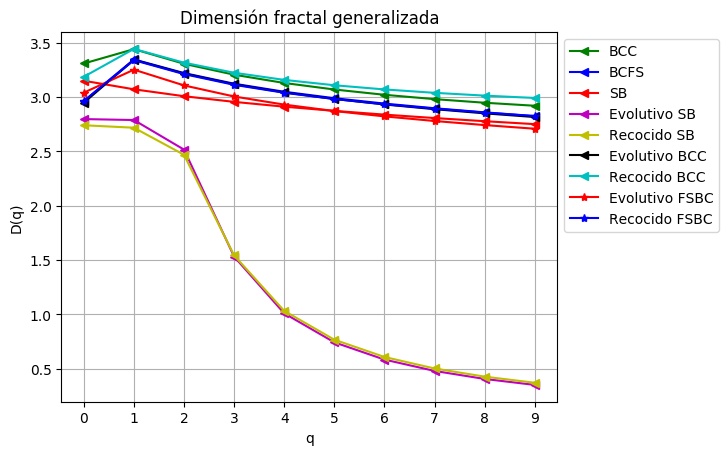
\includegraphics[scale=0.5]{CapituloAAnexos/imagenesAnexoC/Fractalidad/grafica_Dq20180508_231031Random3373Nodes5978.png}
    \caption{Análisis multifractal red aleatoria 3737 nodos}
    \end{minipage}
\end{figure}



\begin{figure}[!htb]
    \begin{minipage}{0.48\textwidth}
        \centering
        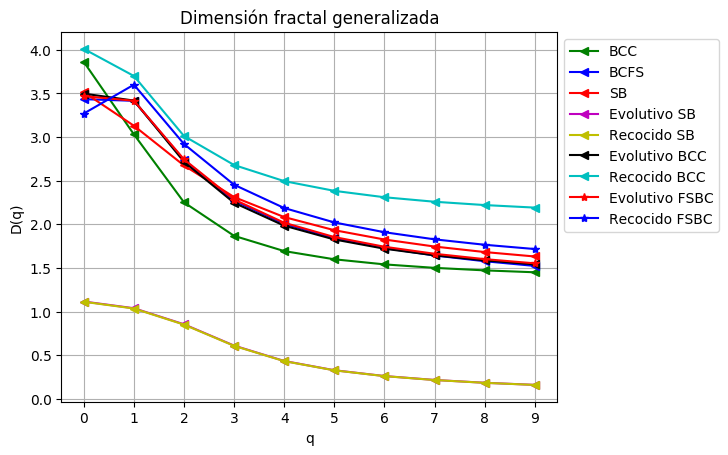
\includegraphics[scale=0.5]{CapituloAAnexos/imagenesAnexoC/Fractalidad/grafica_Dq20180504_000006EColi.png}
        \caption{Análisis multifractal red observada ECOLI}
    \end{minipage}\hfill
   \begin{minipage}{0.48\textwidth}
         \centering
        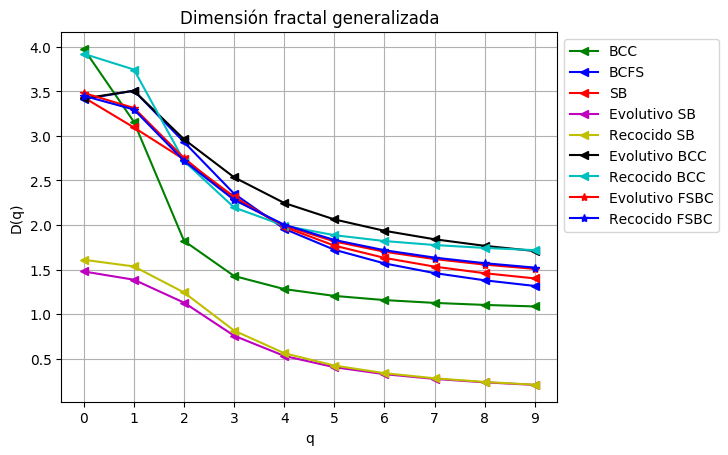
\includegraphics[scale=0.5]{CapituloAAnexos/imagenesAnexoC/Fractalidad/grafica_Dq20180504_010629Celengs.png}
    \caption{Análisis multifractal red observada Celengs}
    \end{minipage}
\end{figure}

\begin{figure}[H]
        \centering
        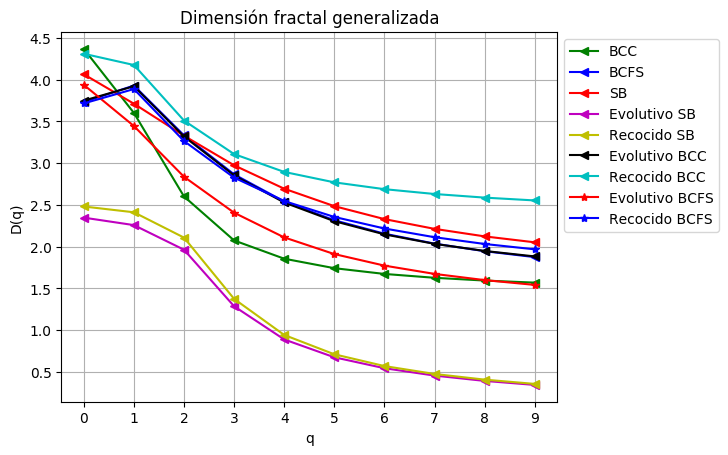
\includegraphics[scale=0.5]{CapituloAAnexos/imagenesAnexoC/Fractalidad/grafica_Dq20180508_182332cerevisiae.png}
        \caption{Análisis multifractal red observada Cerevisiae}
\end{figure}


\begin{figure}[!htb]
    \begin{minipage}{0.48\textwidth}
        \centering
        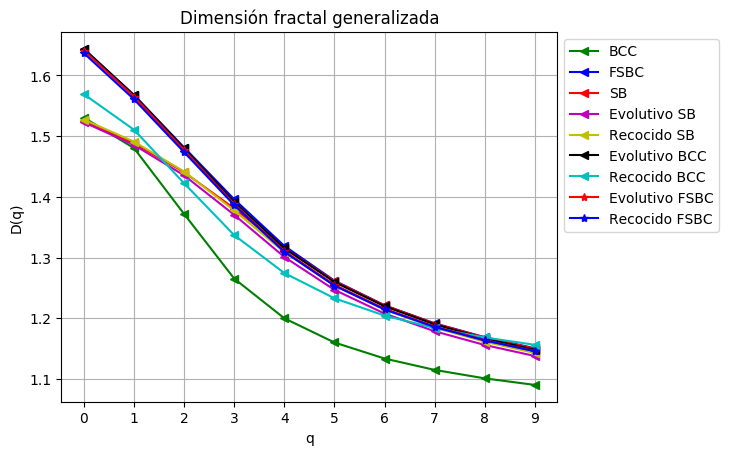
\includegraphics[scale=0.5]{CapituloAAnexos/imagenesAnexoC/Fractalidad/grafica_Dq20180511_101739floweru2v2.png}
        \caption{Análisis multifractal red fractal (2,2)-flower}
    \end{minipage}\hfill
   \begin{minipage}{0.48\textwidth}
         \centering
        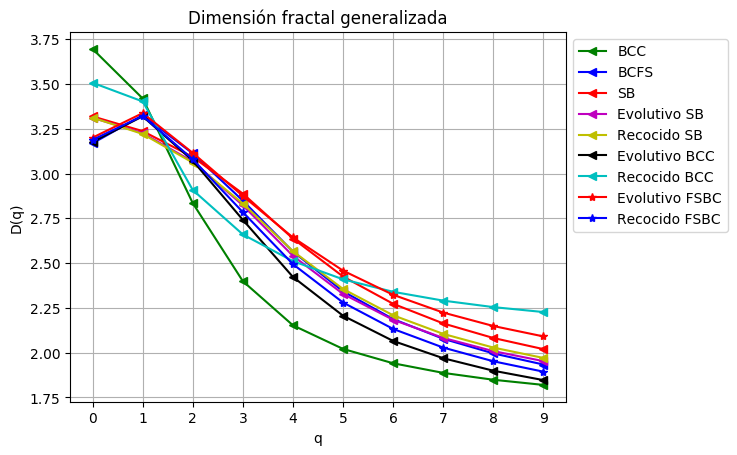
\includegraphics[scale=0.5]{CapituloAAnexos/imagenesAnexoC/Fractalidad/grafica_Dq20180509_000454floweru1v3.png}
    \caption{Análisis multifractal red observada (1,3)-flower}
    \end{minipage}
\end{figure}

\newpage
\subsection*{Resultados análisis de robustez}
\addcontentsline{toc}{subsection}{Resultados análisis de robustez}


\begin{figure}[!htb]
    \begin{minipage}{0.48\textwidth}
        \centering
        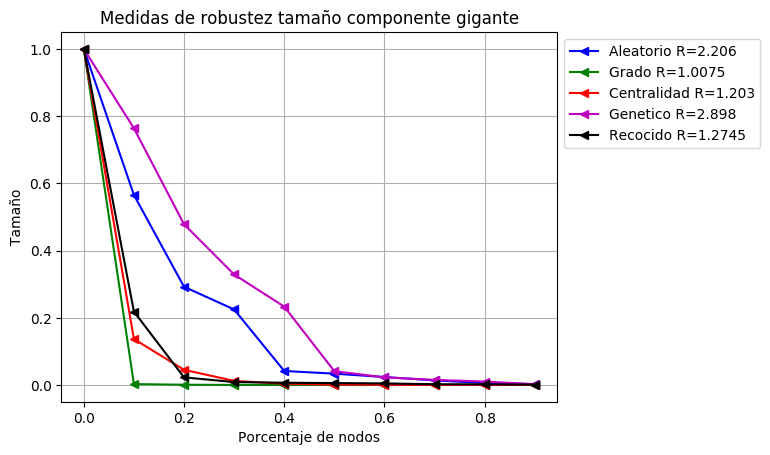
\includegraphics[scale=0.4]{CapituloAAnexos/imagenesAnexoC/Robustez/grafica_GC20180501_030914ScaleFree2000Nodes}
        \caption{Análisis de robustez de red libre de escala de 2000 nodos por tamaño de componente gigante}
    \end{minipage}\hfill
   \begin{minipage}{0.48\textwidth}
         \centering
       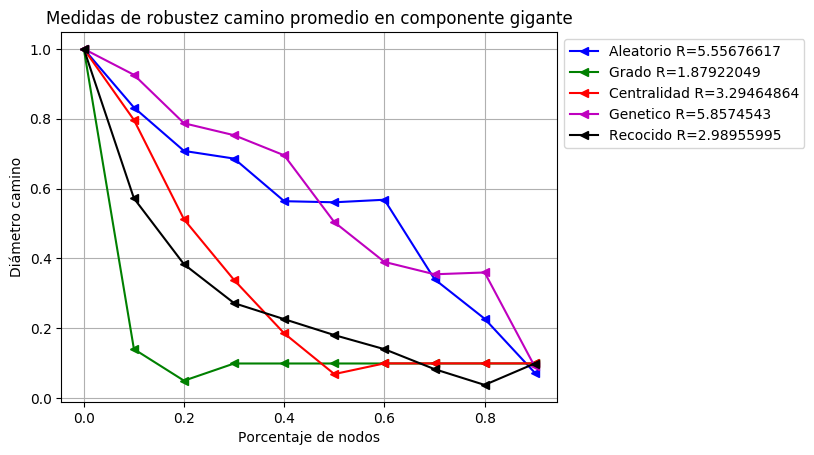
\includegraphics[scale=0.4]{CapituloAAnexos/imagenesAnexoC/Robustez/grafica_APL20180501_030914ScaleFree2000Nodes.png}
        \caption{Análisis de robustez de red libre de escala de 2000 nodos por diámetro de camino más corto}
    \end{minipage}
\end{figure}



\begin{figure}[!htb]
    \begin{minipage}{0.48\textwidth}
        \centering
        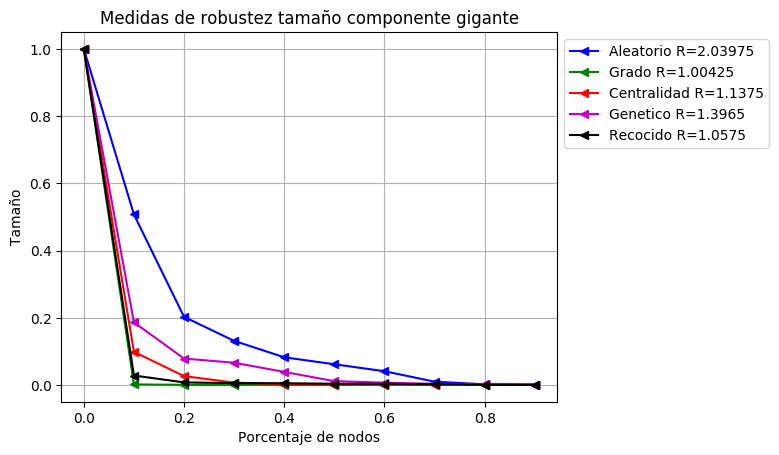
\includegraphics[scale=0.4]{CapituloAAnexos/imagenesAnexoC/Robustez/grafica_GC20180502_060959ScaleFree4000Nodes}
        \caption{Análisis de robustez de red libre de escala de 4000 nodos por tamaño de componente gigante}
    \end{minipage}\hfill
   \begin{minipage}{0.48\textwidth}
         \centering
       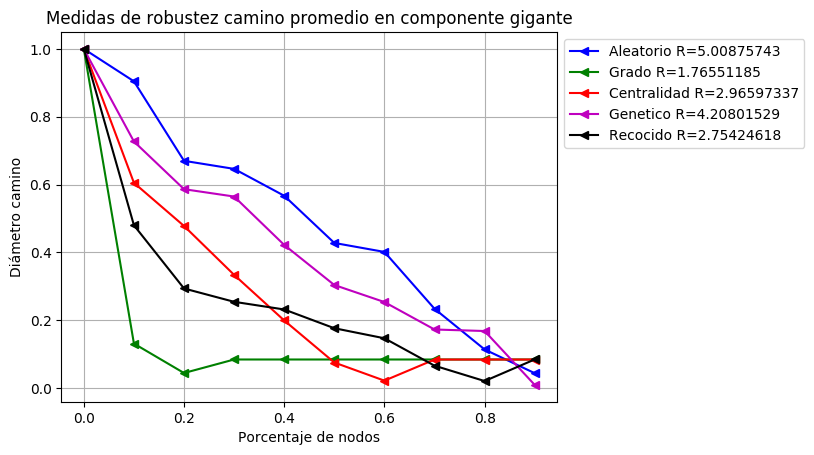
\includegraphics[scale=0.4]{CapituloAAnexos/imagenesAnexoC/Robustez/grafica_APL20180502_060959ScaleFree4000Nodes}
        \caption{Análisis de robustez de red libre de escala de 4000 nodos por diámetro de camino más corto}
    \end{minipage}
\end{figure}


\begin{figure}[!htb]
    \begin{minipage}{0.48\textwidth}
        \centering
        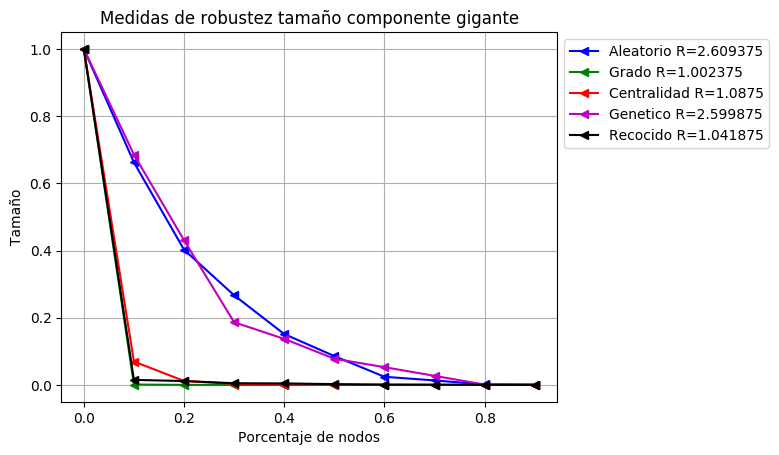
\includegraphics[scale=0.4]{CapituloAAnexos/imagenesAnexoC/Robustez/grafica_GC20180512_143117ScaleFree8000Nodes}
        \caption{Análisis de robustez de red libre de escala de 8000 nodos por tamaño de componente gigante}
    \end{minipage}\hfill
   \begin{minipage}{0.48\textwidth}
         \centering
       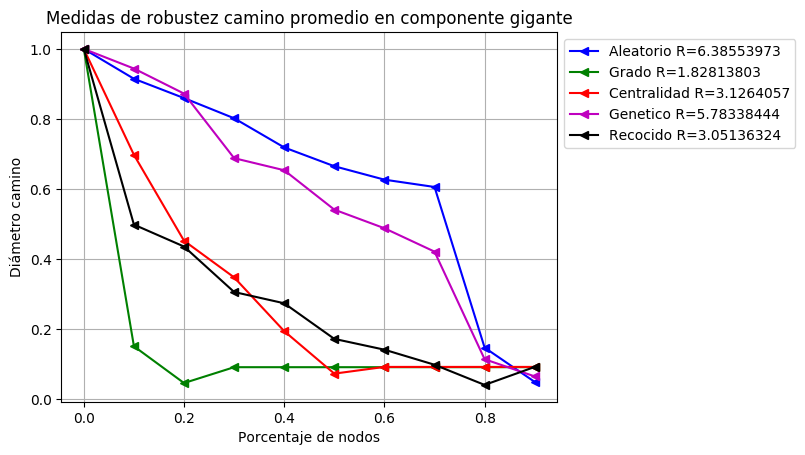
\includegraphics[scale=0.4]{CapituloAAnexos/imagenesAnexoC/Robustez/grafica_APL20180512_143117ScaleFree8000Nodes}
        \caption{Análisis de robustez de red libre de escala de 0000 nodos por diámetro de camino más corto}
    \end{minipage}
\end{figure}



\begin{figure}[!htb]
    \begin{minipage}{0.48\textwidth}
        \centering
        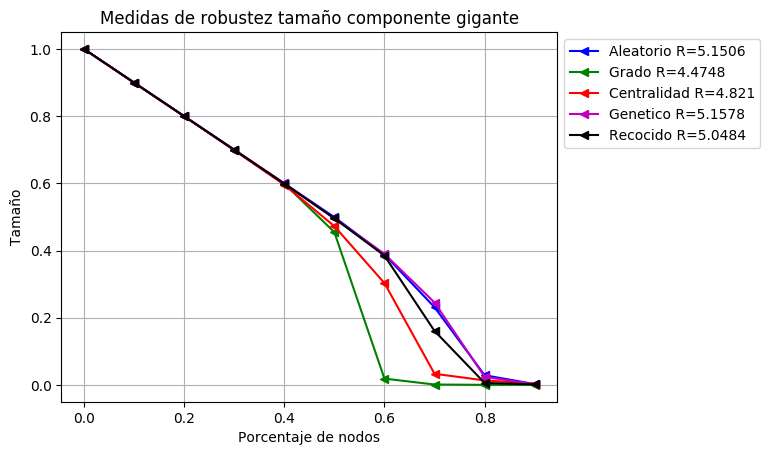
\includegraphics[scale=0.4]{CapituloAAnexos/imagenesAnexoC/Robustez/grafica_GC20180510_143549SmallWorld5000NodesRewire01}
        \caption{Análisis de robustez de red de mundo pequeño de 5000 nodos con p=10\% tamaño de componente gigante}
    \end{minipage}\hfill
   \begin{minipage}{0.48\textwidth}
         \centering
       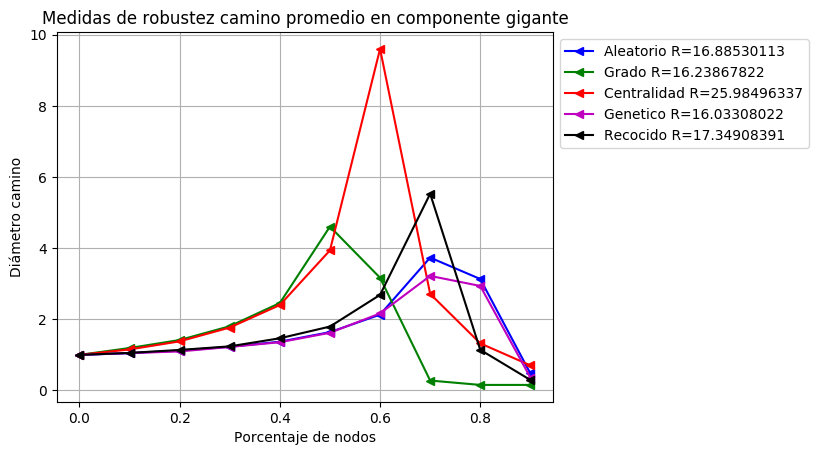
\includegraphics[scale=0.4]{CapituloAAnexos/imagenesAnexoC/Robustez/grafica_APL20180510_143549SmallWorld5000NodesRewire01}
        \caption{Análisis de robustez de red de mundo pequeño de 5000 nodos con p=10\% por diámetro de camino más corto}
    \end{minipage}
\end{figure}

\begin{figure}[!htb]
    \begin{minipage}{0.48\textwidth}
        \centering
        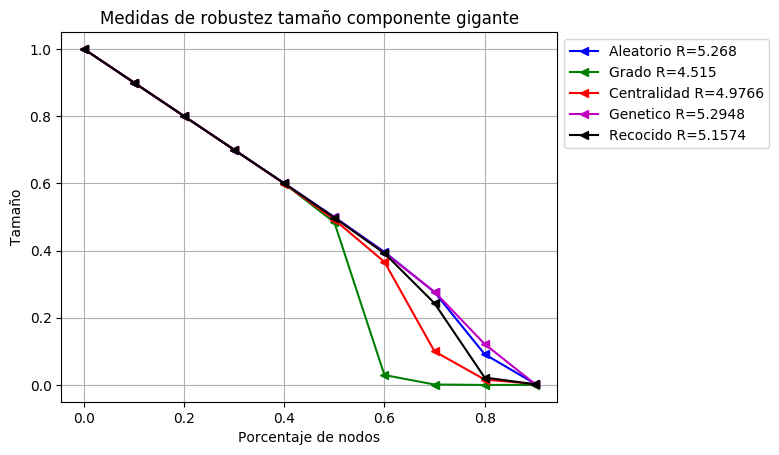
\includegraphics[scale=0.4]{CapituloAAnexos/imagenesAnexoC/Robustez/grafica_GC20180509_105905SmallWorld5000NodesRewire02}
        \caption{Análisis de robustez de red de mundo pequeño de 5000 nodos con p=20\% tamaño de componente gigante}
    \end{minipage}\hfill
   \begin{minipage}{0.48\textwidth}
         \centering
       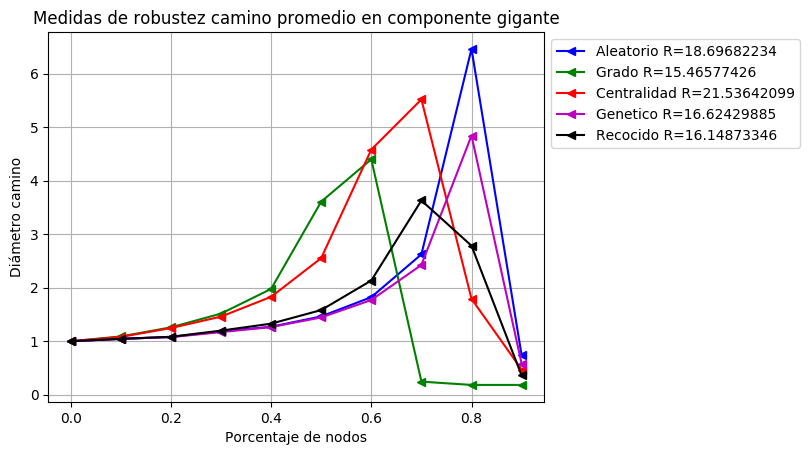
\includegraphics[scale=0.4]{CapituloAAnexos/imagenesAnexoC/Robustez/grafica_APL20180509_105905SmallWorld5000NodesRewire02}
        \caption{Análisis de robustez de red de mundo pequeño de 5000 nodos con p=20\% por diámetro de camino más corto}
    \end{minipage}
\end{figure}



\begin{figure}[!htb]
    \begin{minipage}{0.48\textwidth}
        \centering
        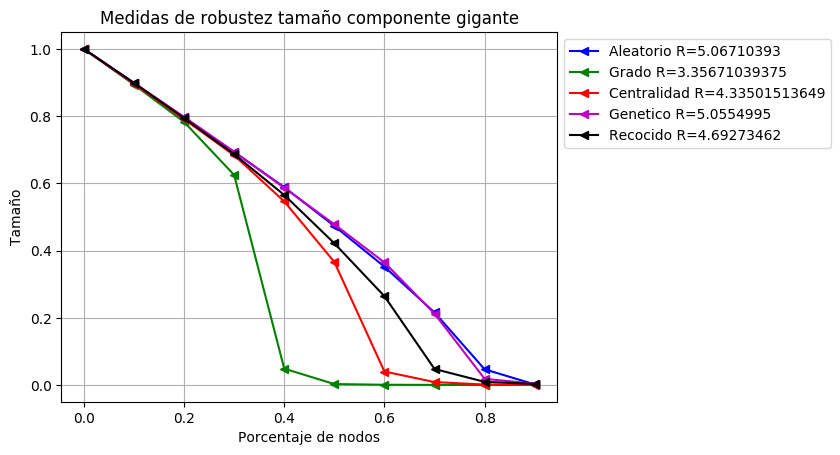
\includegraphics[scale=0.4]{CapituloAAnexos/imagenesAnexoC/Robustez/grafica_GC20180501_072543Random1991Nodes5939}
        \caption{Análisis de robustez de red aleatoria con 1991 nodos por tamaño de componente gigante}
    \end{minipage}\hfill
   \begin{minipage}{0.48\textwidth}
         \centering
       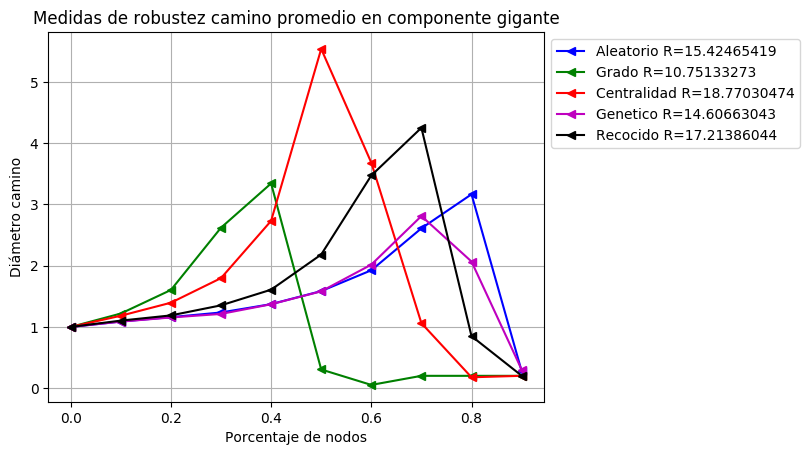
\includegraphics[scale=0.4]{CapituloAAnexos/imagenesAnexoC/Robustez/grafica_APL20180501_072543Random1991Nodes5939}
        \caption{Análisis de robustez de red aleatoria con 1991 nodos por diámetro de camino más corto}
    \end{minipage}
\end{figure}

\begin{figure}[!htb]
    \begin{minipage}{0.48\textwidth}
        \centering
        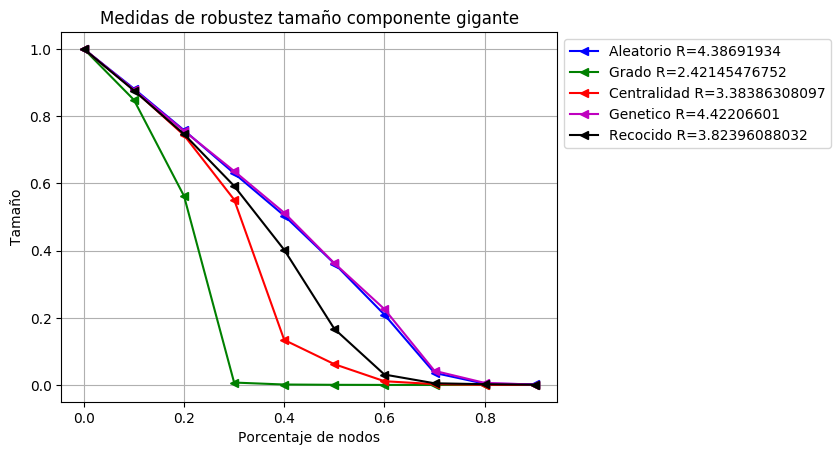
\includegraphics[scale=0.4]{CapituloAAnexos/imagenesAnexoC/Robustez/grafica_GC20180505_190832Random3373Nodes5978}
        \caption{Análisis de robustez de red aleatoria con 3373 nodos por tamaño de componente gigante}
    \end{minipage}\hfill
   \begin{minipage}{0.48\textwidth}
         \centering
       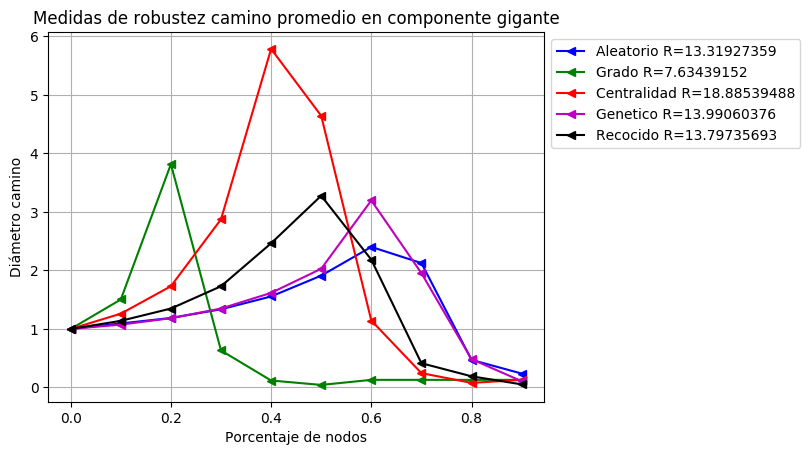
\includegraphics[scale=0.4]{CapituloAAnexos/imagenesAnexoC/Robustez/grafica_APL20180505_190832Random3373Nodes5978}
        \caption{Análisis de robustez de red aleatoria con 3373 nodos por diámetro de camino más corto}
    \end{minipage}
\end{figure}

\begin{figure}[!htb]
    \begin{minipage}{0.48\textwidth}
        \centering
        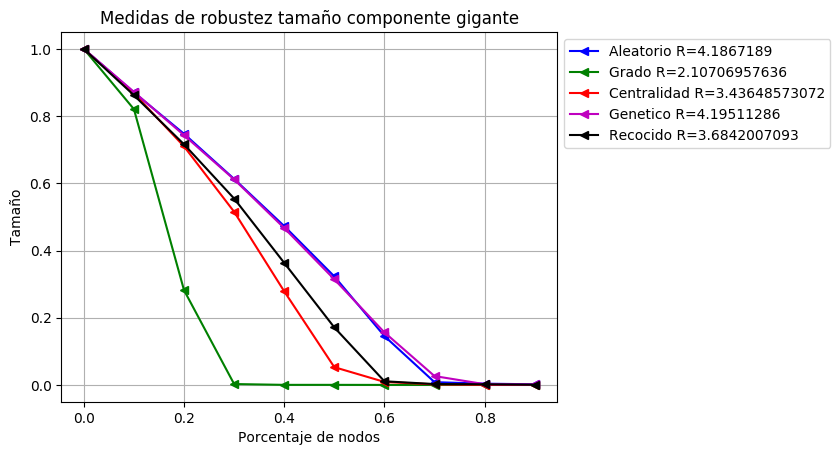
\includegraphics[scale=0.4]{CapituloAAnexos/imagenesAnexoC/Robustez/grafica_GC20180512_015627Random5620Nodes8804}
        \caption{Análisis de robustez de red aleatoria con 5620 nodos por tamaño de componente gigante}
    \end{minipage}\hfill
   \begin{minipage}{0.48\textwidth}
         \centering
       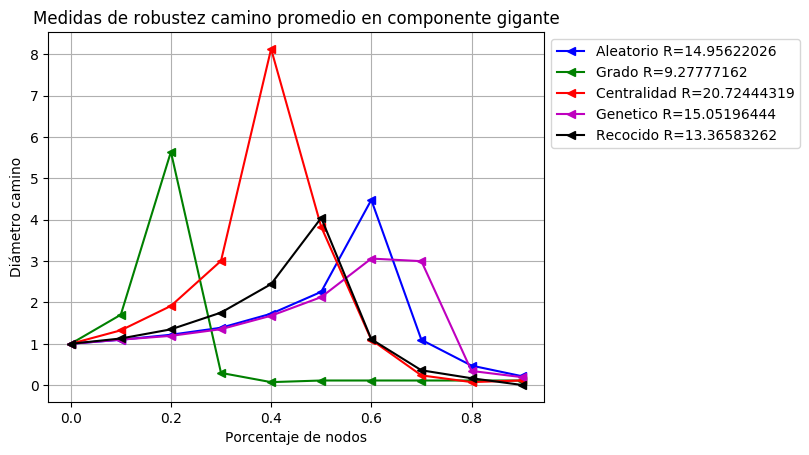
\includegraphics[scale=0.4]{CapituloAAnexos/imagenesAnexoC/Robustez/grafica_APL20180512_015627Random5620Nodes8804}
        \caption{Análisis de robustez de red aleatoria con 5620 nodos por diámetro de camino más corto}
    \end{minipage}
\end{figure}


\begin{figure}[!htb]
    \begin{minipage}{0.48\textwidth}
        \centering
        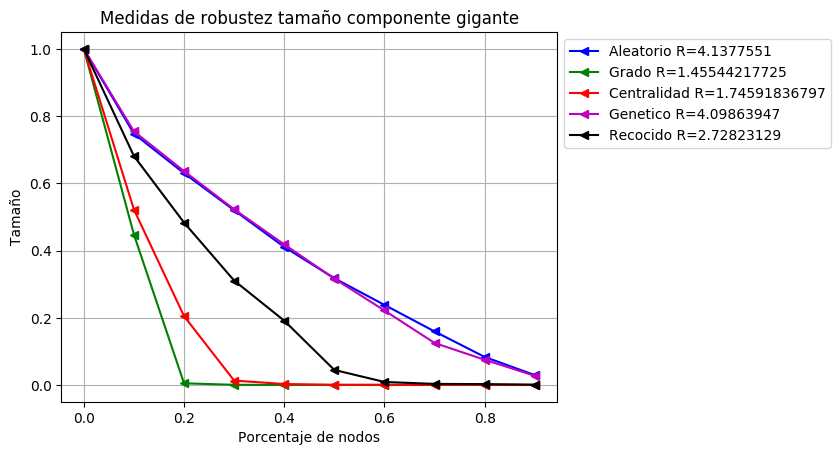
\includegraphics[scale=0.4]{CapituloAAnexos/imagenesAnexoC/Robustez/grafica_GC20180506_091444EColi}
        \caption{Análisis de robustez de red observada Ecoli por tamaño de componente gigante}
    \end{minipage}\hfill
   \begin{minipage}{0.48\textwidth}
         \centering
       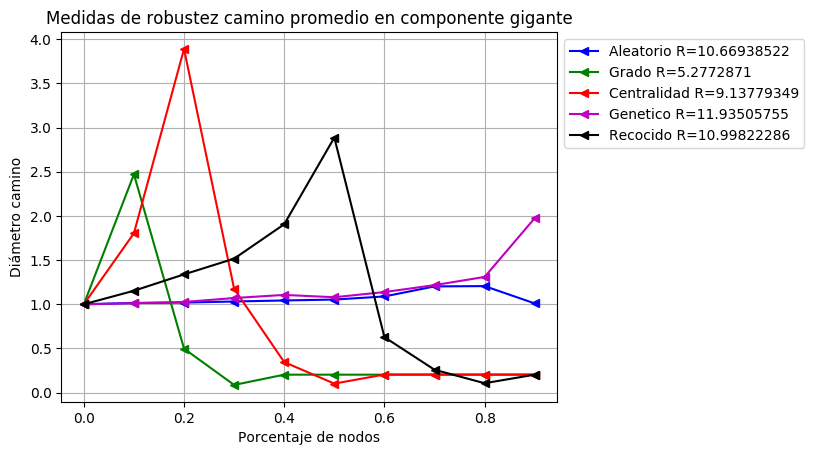
\includegraphics[scale=0.4]{CapituloAAnexos/imagenesAnexoC/Robustez/grafica_APL20180506_091444EColi}
        \caption{Análisis de robustez de red observada Ecoli por diámetro de camino más corto}
    \end{minipage}
\end{figure}


\begin{figure}[!htb]
    \begin{minipage}{0.48\textwidth}
        \centering
        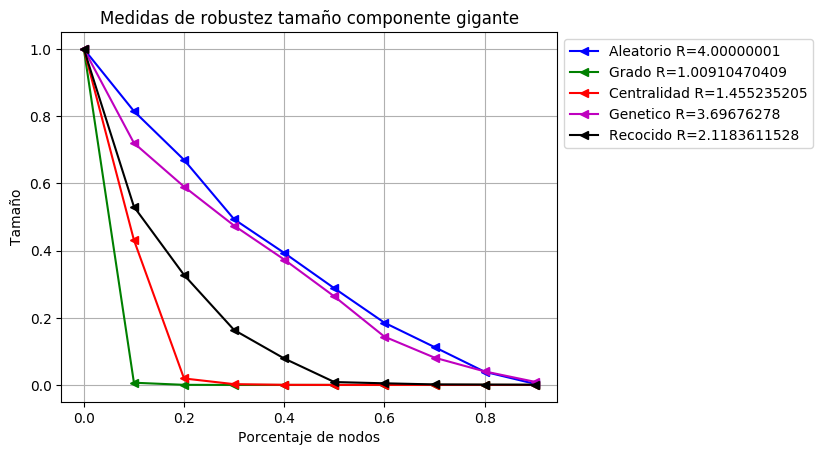
\includegraphics[scale=0.4]{CapituloAAnexos/imagenesAnexoC/Robustez/grafica_GC20180508_020345Celengs}
        \caption{Análisis de robustez de red observada Celegens por tamaño de componente gigante}
    \end{minipage}\hfill
   \begin{minipage}{0.48\textwidth}
         \centering
       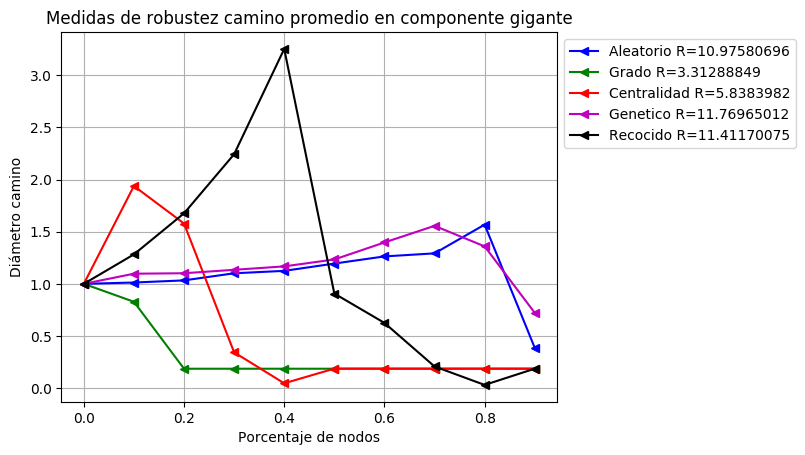
\includegraphics[scale=0.4]{CapituloAAnexos/imagenesAnexoC/Robustez/grafica_APL20180508_020345Celengs}
        \caption{Análisis de robustez de red observada Celegens por diámetro de camino más corto}
    \end{minipage}
\end{figure}

\begin{figure}[!htb]
    \begin{minipage}{0.48\textwidth}
        \centering
        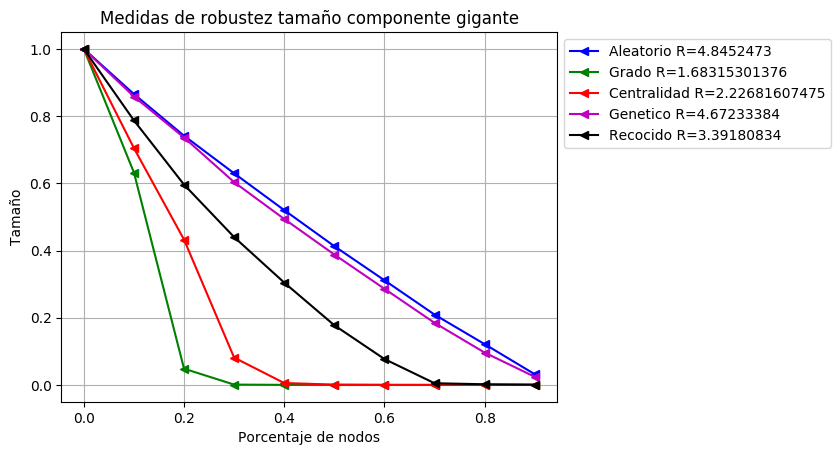
\includegraphics[scale=0.4]{CapituloAAnexos/imagenesAnexoC/Robustez/grafica_GC20180510_203826cerevisiae}
        \caption{Análisis de robustez de red observada Cerevisae por tamaño de componente gigante}
    \end{minipage}\hfill
   \begin{minipage}{0.48\textwidth}
         \centering
       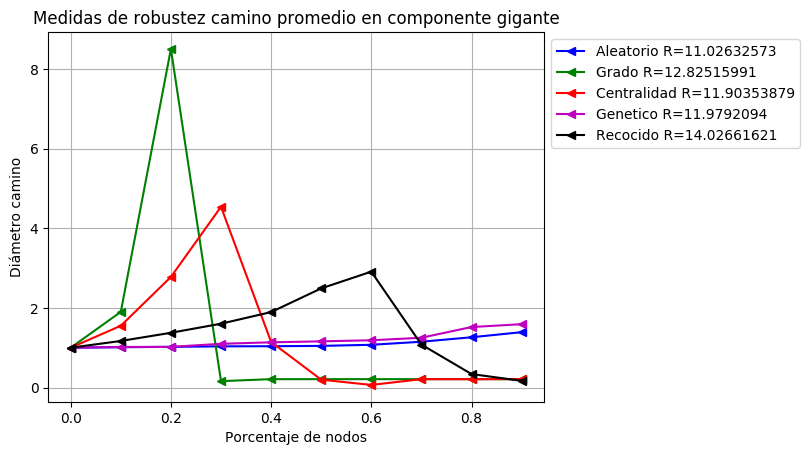
\includegraphics[scale=0.4]{CapituloAAnexos/imagenesAnexoC/Robustez/grafica_APL20180510_203826cerevisiae}
        \caption{Análisis de robustez de red observada Cerevisae por diámetro de camino más corto}
    \end{minipage}
\end{figure}


\begin{figure}[!htb]
    \begin{minipage}{0.48\textwidth}
        \centering
        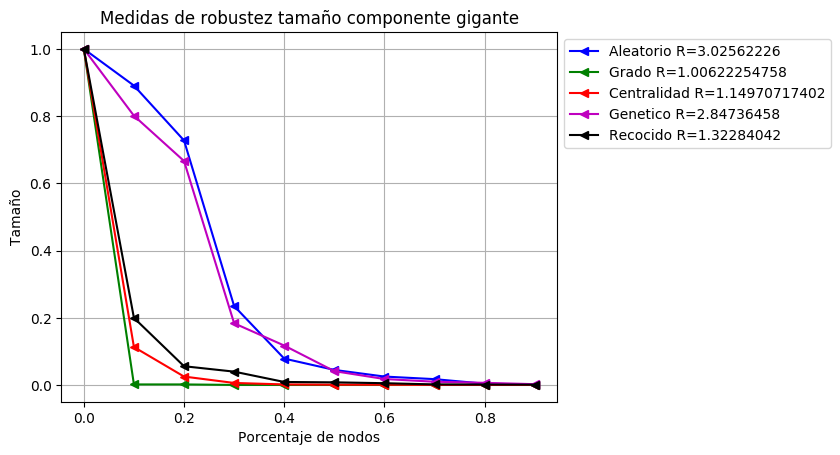
\includegraphics[scale=0.4]{CapituloAAnexos/imagenesAnexoC/Robustez/grafica_GC20180505_044516floweru2v2}
        \caption{Análisis de robustez de red fractal (2,2)-flower por tamaño de componente gigante}
    \end{minipage}\hfill
   \begin{minipage}{0.48\textwidth}
         \centering
       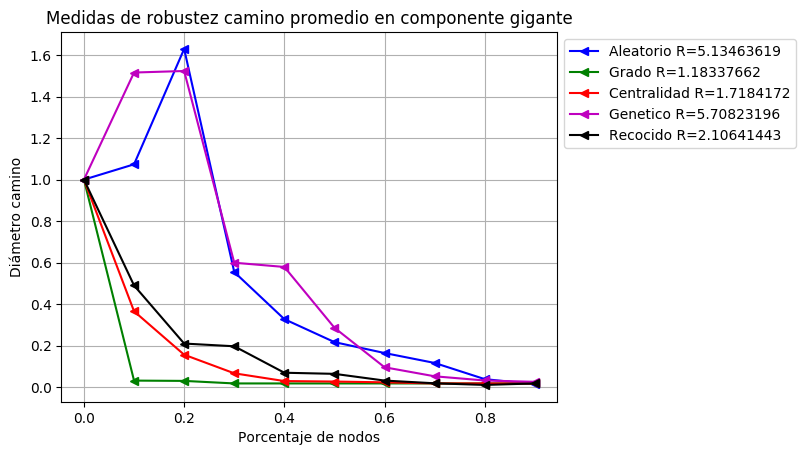
\includegraphics[scale=0.4]{CapituloAAnexos/imagenesAnexoC/Robustez/grafica_APL20180505_044516floweru2v2}
        \caption{Análisis de robustez de red fractal (2,2)-flower por diámetro de camino más corto}
    \end{minipage}
\end{figure}


\begin{figure}[!htb]
    \begin{minipage}{0.48\textwidth}
        \centering
        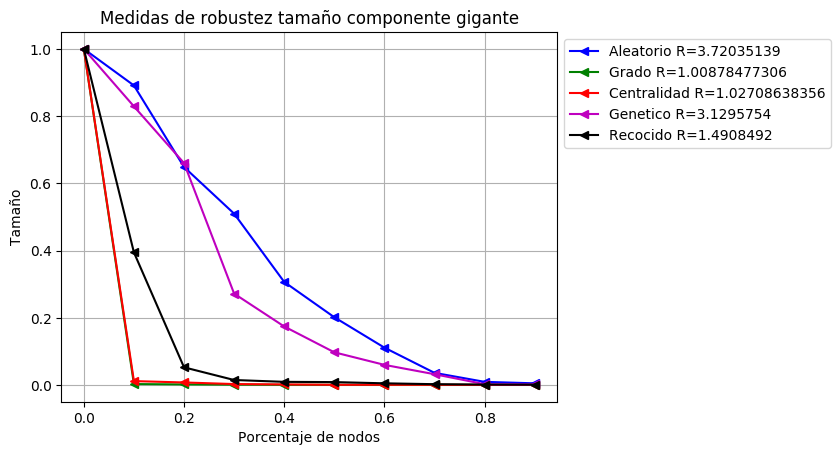
\includegraphics[scale=0.4]{CapituloAAnexos/imagenesAnexoC/Robustez/grafica_GC20180501_151350floweru1v3}
        \caption{Análisis de robustez de red fractal (1,3)-flower por tamaño de componente gigante}
    \end{minipage}\hfill
   \begin{minipage}{0.48\textwidth}
         \centering
       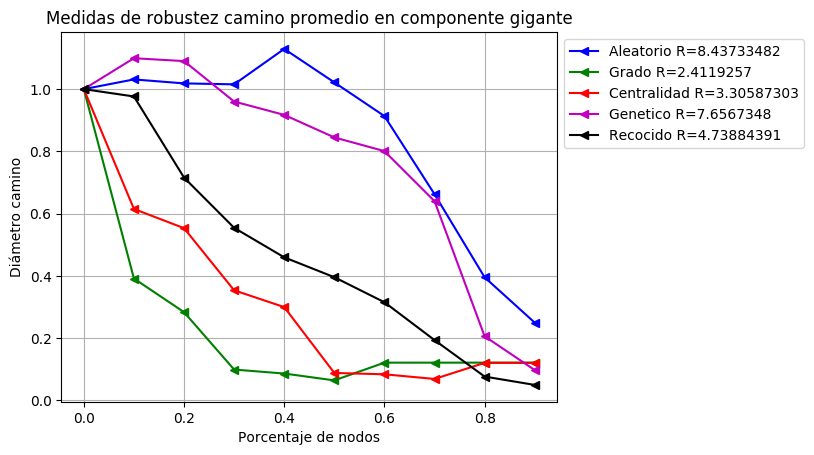
\includegraphics[scale=0.4]{CapituloAAnexos/imagenesAnexoC/Robustez/grafica_APL20180501_151350floweru1v3}
        \caption{Análisis de robustez de red fractal (1,3)-flower por diámetro de camino más corto}
    \end{minipage}
\end{figure}


%\subsection*{Resultados análisis de multifractalidad y robustez}
%\addcontentsline{toc}{subsection}{Resultados análisis de multifractalidad y robustez}